\documentclass[10pt,conference,compsocconf]{IEEEtran}

\usepackage{hyperref}
\usepackage{graphicx}
\usepackage{xcolor}
\usepackage{blindtext, amsmath, comment, subfig, epsfig }
\usepackage{grffile}
\usepackage{caption}
\usepackage{multirow}
%\usepackage{subcaption}
\usepackage{algorithmic}
\usepackage[utf8]{inputenc}


\title{CS-523 SecretStroll Report}
\author{Manon Michel, Tom Demont}
\date{April 2022}

\begin{document}

\maketitle


\section{Introduction}
Location data are of the most sensitive information. Their high dimensionality and intrinsic binding to person-hood require to deal carefully with this asset. This makes Point of Interest (PoI) recommendation based on location a very sensitive application requiring careful design at every step. We therefore, in this project, try to model, attack and defend privacy preserving mechanisms on top of this toy application through its authentication system, its data storage and its network communication.

\section{Attribute-based credential}
\subsection{System's attributes}
First, we analysed the authorizations our system wants to propose. From the handout, we came to the conclusion that each subscription should require a specific authorization. Indeed, a user should be able to take any subset of subscriptions in a regular "pay per subscription" model as it is described. This would allow us to disclose only the minimum required for each query: we disclose only the attributes corresponding to the PoI types we want to query for, letting the user choose the minimum number of subscriptions required per query and not linking to an identity.

We can also note that we took care of discarding the no-subscription case: we decided to not authorize a user to subscribe to nothing as it would make no sense even in a regular subscription model. This avoids useless computations and having users making queries for nothing which could generate a cost. Nonetheless, the anonymous credential system we implemented could support it without the input verification made.

We also chose not to include the username in the attributes in order to better ensure unlinkability.

Finally, as suggested, we also added as attribute a unique random number (random object of class \texttt{Bn} to have low collision probability). This one is usually not shown to the issuer or verifier (as it would break the desired unlinkability with subsequent showings) but can reveal to be useful in some critical operations. Indeed, we could imagine judicial circumstances where some party would like to assert that they did not steal another's credential. They could do so by showing their hidden unique user attribute.
\subsection{Mapping to the \texttt{AttributeMap}}
\subsubsection{Attribute representation}
Considering the above discussion, we made choices for attributes accordingly. We decided to represent our attributes by \texttt{Bn} of the \texttt{petrelic.bn} class. This makes computations in \texttt{credential.py} very handy as we can directly run computations on the attributes by using them as exponents of $G_1$ elements as described in the ABC guide. We must note that we'll only manipulate numbers modulo $|G_1|$ (noting that on our curves, $|G_1|=|G_2|=|G_T|$). Indeed, this serves 2 purposes: first, for serialization, \texttt{petrelic} requires strictly positive \texttt{Bn}. Secondly, the security of our system requires manipulation of numbers modulo the order of the used group. Notably, in the proofs of knowledge, the prover sends the responses corresponding to the challenge, those must be sent modulo $|G_1|$ if we do not want an observer having the challenge to deduce information about the secret value. We made sure to hold modulo $|G_1|$ values at conversions from string/bytes or at the construction of the objects holding those values that we defined (\texttt{SecretKey}, \texttt{PublicKey}, \texttt{PedersonKnowledgeProof}).

\subsubsection{From string/bytes to the attribute}
In the system's initialization, the server's recognized subscriptions are received as strings. From the run examples, those are human readable names representing the names of the classes of points of interest. To represent those as bytes, we can easily use \texttt{.encode()}. We here made the decision to also hash this bytes representation of attribute string. Indeed, we wanted to make it cryptographically hard to find a collision between integer values of attributes so that an adversary have little hope to find 2 attribute values that have the same attribute representation and therefore, tweak the system into paying a low cost subscription colliding with another expensive one. Finally, we use the \texttt{Bn.from\_binary()} function to have a BigNumber. As explained above, we then put our big number modulo $|G_1|$ and that this function is not strictly one to one as the size of $|G_1|$ is limited but considering the number of meaningful subscriptions name that is very limited (there are at most around a million of English words\cite{noauthor_how_2020}), this is acceptable to us. This also makes non-necessary the need for hash function as explained above, but in order to avoid a Telegram-like crypto argument, we preferred to go for the most secure way. 
\subsubsection{\texttt{AttributeMap} object}
Our \texttt{AttributeMap} object is therefore represented by a \texttt{dict} mapping an integer to the value of our attribute. We made the choice to always, in a system with $L$ subscriptions (decided by the server at initialization), give a credential to a user for $L+1$ attributes: the first one being the random identifier and the others being either the \texttt{Bn} representation of the PoI subscription name, or the \texttt{Bn} representation of the string "None", representing the fact that a user is not subscribed to this PoI. This allows us to easily verify paid subscriptions on showing: if the user can show a valid credential for a PoI subscription name, they can access the service, if they show a valid credential but for None, they can be refused, if they show a non valid credential, this should be verifiable by the proof of knowledge. In a system where subscriptions are "restaurant", "park" and "hotel" and we have a user subscribed to "park" and "hotel" only, the corresponding \texttt{AttributeMap} would be:
\begin{center}
\begin{tabular}{||c c||} 
 \hline
 Attr index & Value \\ [0.5ex] 
 \hline\hline
 1 & a random \texttt{Bn} \\ 
 \hline
 2 & \texttt{Bn(sha256("None"))} \\
 \hline
 3 & \texttt{Bn(sha256("park"))} \\
 \hline
 4 & \texttt{Bn(sha256("hotel"))} \\
 \hline
\end{tabular}
\end{center}
This object presents the double advantage of not leaking, by its length, the number of subscriptions a user had taken (assuming all Bn are represented by the same number of bytes) while being very convenient to manipulate for computations. Indeed, we always have access to the pair index,value, allowing the verifier to get the index of the correct $Y_i$ public key value along with the $a_i$ attribute value (with notations from the ABC credentials guide).
\subsection{Going non-interactive}
After defining the attributes and our credential with the PS scheme, we finally re-define our proofs of knowledge. Consider the fact that our secrets are, in both proofs, bounded to equations defined by the product of some group elements known to both parties ($Y_i$ or $e(\sigma',\Tilde{Y}_i)$ for example) raised to the power of our secrets ($t$ or $a_i$). This naturally brings the Pedersen commitment scheme to mind. We therefore implemented our proofs of knowledge following this idea as described in the Exercise Set 1.2 Solutions\cite{exercise_set_1.2}. We extended it to make it non-interactive using the Fiat-Schamir heuristic: instead of requiring the server to send a challenge, we computed it as a hash of the public values, the commit value (denoted \texttt{com} in the exercise and the code) and the prover commitment (denoted $R$ in the exercise and code). 

Therefore, the prover no longer sends $R$ and the responses $s_i$ but only the generated challenge $c$ and the responses $s_i$. The changes induced on the verifier side is that they now have to compute the commit value $R$ with the given information (as they would do in the interactive case) and use this value to compute the challenge $c'$. The verification is now the check that $c=c'$ which should be hard to forge for a prover not having a valid credential as $c$ would be binded to $R$ and \texttt{com} that depend on this credential. Note that we decided, in this report and in the code, to rather call the proof a "proof of knowledge" rather than a "zero knowledge proof" due to the fact that using the Fiat-Schamir heuristic, we break the zero-knowledge property by making non-simulatable the trace corresponding to the proof (a non-holder of the secret cannot make believe they have it by producing valid $c$ and $s_i$).

Finally, there are slight differences between both knowledge proofs that we may want to notice:
\subsubsection{} In the proof of holding user attributes to blindly sign, the challenge is computed as $c=H(g,Y_1,...,\Tilde{Y_L},\texttt{com},R)$. This is very close to the implementation detailed in Exercise Set 1.2 \cite{exercise_set_1.2}
\subsubsection{} In the second proof, we took advantage of the nature of the commit value to avoid sending it (this does not change the cryptographic security of our proof but is just a convenience that reduces the communication cost). Indeed, in the ABC guide, showing protocol part 2.b, the left hand side of the equation happens to be computable using only disclosed attributes, public values and showed credential which allows the server to compute it without receiving it directly. The right hand side is computable using public values, showed credential and hidden attributes which makes it computable by the prover. Doing so allows to have the complete equation (both left and right hand side are computed independently, requiring the equation to hold for the proof to succeed) and avoids sending a redundant \texttt{com} value. Finally, we noted that it might be useful to require the credential showing knowledge proof to be binded to the actual location query. This reduces the hash collision probability as augmenting the entropy of the hashed material and also requires the adversary to have access to the location query which can be seen as requiring a stronger adversary. Therefore, the final challenge is computed as $c=H(g,Y_1,...,\Tilde{Y_L},\texttt{com},R,\texttt{message})$ where \texttt{message} contains the location query text.

\subsection{Test}
We tested our code with tests that we wrote in 2 files: \texttt{test\_credential.py} and \texttt{test\_stroll.py}. We used the handy test framework proposed by pytest and made test function for every function in \texttt{credential.py} and \texttt{stroll.py}. The test for the credential system aims to be quite generic while the stroll system tests are rather driven toward concrete utilization. The main points to note for the credential systems tests are the use of parameters to determine the possible range for attributes generation: \texttt{MIN\_NB\_ATTRIBUTES} and \texttt{MAX\_NB\_ATTRIBUTES} so that we can test different settings under varying amount of subscriptions. The attributes are randomly generated in order to avoid having deterministic inputs. Finally, we tested many failing cases with badly formed attribute maps, fake keys, bad user states and also took care of randomly shuffling between the user and issuer or hidden and showed attributes. For the stroll system tests, we took care of testing the serialization (as we first had some issues with it). After that, we tested every sub-functionality by putting some predetermined subscriptions (close to the ones proposed in the \texttt{README.md} of the handout). Both fully succeeding paths are made with a different number of available subscriptions and for different user subscriptions to avoid success binded to particular server conditions. We took care in the failing path to simulate an adversary trying to escalate their privilege and show a token for subscription they didn't pay for or subscribe to PoI types that do not exist. A last note of tests is that we worked with GitHub CI and created a workflow of tests, to help us develop confidently, that you can find as \texttt{docker-stroll-system.yml} and \texttt{pytest-tests.yml} that made sure our tests passed and the system were working on every action on the repository.

To assess the quality of our tests, we thought about making use of code coverage to make sure we reach the edge cases we deal with in our tests. We tried to run this with the module \texttt{pytest-coverage}, you can find the results in the folder \texttt{htmlreport}. Essentially, we obtained 96\% coverage for \texttt{credential.py} and 94\% coverage for \texttt{stroll.py}. 
\subsection{Evaluation}

To evaluate the performances, we made use of the module \texttt{pytest-benchmark}.

The \texttt{stroll.py} benchmark tests the following features: key generation, issuance, signing and verification given 2 and 4 attributes. The performance results can be found in Table \ref{tab:strollperf} given two different architectures. 


\begin{table}[h!]
\centering
\begin{tabular}{ |c|c|c|c| } 
\hline
\ stat & step & arm64 4 cores & x86\_64 2 cores\\
\hline
\hline
\multirow{4}{4em}{mean} & key generation & 1.5647 & 3.0910 \\ 
& issuance & 7.6928 & 18.8247 \\ 
& signing & 10.1355 & 14.5832 \\ 
& verification\_2 & 9.3371 & 14.5389 \\ 
& verification\_4 & 12.4915 & 18.3777 \\
\hline
\multirow{4}{4em}{std} & key generation & 0.0588 & 0.8270 \\ 
& issuance & 0.3774 & 9.3719 \\ 
& signing & 0.2248 & 1.7943 \\ 
& verification\_2 & 0.3390 & 2.4759 \\ 
& verification\_4 & 0.4875 & 4.1691 \\ 
\hline
\end{tabular}
\caption{\label{tab:strollperf}Speed in Milliseconds (ms) }
\end{table}


\begin{table}[h!]
\centering
\begin{tabular}{ |c|c| } 
\hline
item & bytes \\
\hline
\hline
secret key & 689 \\ 
public key & 2168 \\ 
issue request & 623 \\
blind signature & 769 \\ 
credential & 919 \\ 
disclosure proof & 994 \\ 
\hline
\end{tabular}
\caption{Communication costs (bytes)}
\end{table}
Details of benchmarks can be found in the \texttt{.benchmarks} folder (also including nice visual histograms).
\section{(De)Anonymization of User Trajectories}

\subsection{Privacy Evaluation}

In order to exploit the given data, we first decided to provide some improvements. First of all, we modified the timestamps, which were originally floats ranging from 0.622 to 465.997 (hours from the beginning of the simulated data capture, on a midnight between a Sunday and a Monday). We first rounded them and took the value modulo 24 in order to only keep the corresponding hour of the day (0 to 24). We also used the original timestamps to obtain the corresponding day type (i.e. week-day or week-end).

With this more explicit timestamp information, we can filter frequent locations according to week-ends and nights (most likely home) and week-days during working hours (most likely work location). We could therefore perform a de-anonymization attack by identifying the home and work location for each user under the assumption that these two pieces of information are often sufficient to uniquely identify somebody. We therefore use the IP address to identify separate users and latitude, longitude and timestamps to identify their home and work location. For this we extract each precise location detected for each user along with their frequency along the separate time-frames (work or home). 

The data we use in this attack is data that is available on the server side, we therefore consider an adversarial model such as the service provider. In this attack we assume that most people work between 8-17h from Monday to Friday and most people are at home between 21h-6h or from Saturday to Sunday.  

\subsection{Defences}

\subsubsection{Location Generalization}
POI queries from users are stored on the server side with precise location (represented by the latitude and longitude). The area is divided into sub sections by a grid and each of these subsections is identified by an integer value, the grid cell id. In order to return the requested POIs to the user, the server will find the grid cell id corresponding to their precise location. One can thus note that storing the precise location of users on the server-side brings nothing more to the utility than directly storing the grid cell id. We will therefore do this to mitigate the information leaked by the location data. By dealing with the grid id retrieval on the client-side, we aim to put the trust on the client side. It is notably desirable to remove the precise location as the latter reveals information such as trajectories and potentially the identity of the user as work and home locations are often sufficient to uniquely identify people.  

In order to evaluate this defence, we therefore performed the same attack but using grid cells instead of precise coordinates. We achieved this by using the \texttt{location\_to\_cell\_id()} method in grid.py. We then once again filtered and retrieved the top queried location for each user given the home timeframe and the work timeframe. 

In terms of privacy metrics, as our latitude and longitude points are very precise (11 decimal precise places), we can therefore consider that it is accurate to the millimeter (assuming that over eight decimal places is overkill). In the case of grid cell id's, we have a $10\times10$ grid, with a total area size of 0.07 latitude and 0.10 longitude. The range covered by each grid cell is therefore 0.007 latitude and 0.01 longitude. This corresponds to respectively 770m and 1.1km of range. Therefore using grid cells rather than precise location will make a location indistinguishable by at least 770m in latitude and 1.1km in longitude as opposed to 1mm, which represents a considerable generalization.

A second privacy metric is the size of the anonymity set. When using the precise location, if we take the most probable home,work location pair for each ip address, out of 200 different users, only 2 have the same pair, all others have a unique pair which constitutes a very small anonymity set. When using grid cells instead, we have 15 different home,work pairs for which there is more than one associated ip address, which is already a lot better. We provide a more extensive comparison of average anonymity set size in Table \ref{tab:anonset}. Whether we consider location pairs or individual locations, this mitigation considerably improves the average anonymity set size.

\subsubsection{Timestamp Obfuscation}
Timestamps are valuable data but often don't bring much to the utility of application. Such data is useful for attackers, notably in de-anonymization attacks. In the context of our application, the timestamps are not necessary and can therefore be removed. For example, we previously used timestamps to identify which repeated user location corresponds most likely to their home or workplace. 

In order to measure the privacy, we compare the anonymity set size given the timestamp information (i.e. hour of the day and weekend or weekday) with reduced timestamp information (only day type). As can be seen in Table \ref{tab:anonset}, if we take the case where we use precise location data, the average anonymity set size with the full timestamp data is of 1.005 compared to 1.124 with the reduced timestamp information. Given only grid cell id, we go from 1.093 to 3.448. We can therefore conclude that obfuscating timestamp information increases the anonymity set for user location data and therefore is a good defence. 

In reality, we could remove the timestamp entirely but it is harder to measure the privacy impact in terms of our attack as we can not classify the home and work locations without changing the original process which would reduce the significance of our privacy analysis.

\begin{table}[h!]
\centering
\begin{tabular}{ |c|c|c|c| } 
\hline
 &  & \multicolumn{2}{c|}{Avg anonymity set size} \\
 \hline
timestamp & location & grid cells & coordinates\\
\hline
\hline
\multirow{3}{4em}{days and hours} & home,work & 1.093 & 1.005 \\ 
& home & 3.636 & 1.242 \\ 
& work & 5.714 & 3.509 \\ 
\hline
days & home,work & 3.448 & 1.124 \\ 
\hline
\end{tabular}
\caption{\label{tab:anonset}Average anonymity set size}
\end{table}


\section{Cell Fingerprinting via Network Traffic Analysis}

\subsection{Implementation details}
\subsubsection{Trace collection}
We performed the data collection with a shell script using the packet capture package \texttt{tcpdump}\cite{noauthor_tcpdump1_nodate}. We automated the capture of packets for queries over all grid cells ids and made a \texttt{.pcap} file for each capture. Our main ideas were to filter out the packets that are not part of the application behaviour: in order to achieve this we kept only the TCP packets that have a non-empty payload during our communication, discarding TCP control packets and network control (ARP, IP keep alive ...), essentially packets which are not revealing application behaviour. We could not filter per port as the TOR communication changes the port, potentially connecting to different TOR nodes at every session. The details and comments on this are in the script \texttt{capture.sh}. Finally, before extracting features, we collected the length of every trace and performed data cleaning to remove outliers coming from capture issues. To do so, we used the common framework of using the z-score. This evaluates how many standard deviations a record is far from the normalized mean of a column. We removed from the data the records having a z-score greater than 3, yielding better correlation between trace lengths for a same grid cell id. See Fig \ref{fig:lengths_before_cleaning} and \ref{fig:lengths_after_cleaning} for visuals about the cleaning effectiveness.
\begin{figure}
    \centering
    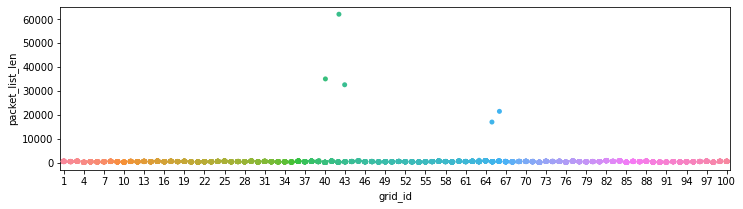
\includegraphics[width=0.4\textwidth]{output2.png}
    \caption{Trace length grouped by grid id before outliers filtering}
    \label{fig:lengths_before_cleaning}
\end{figure}
\begin{figure}
    \centering
    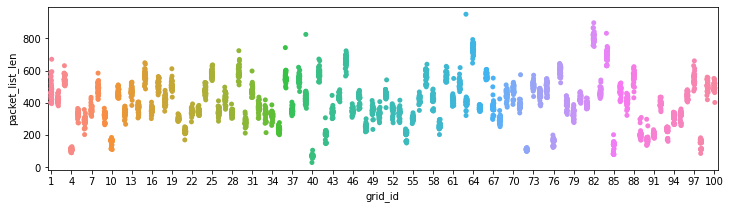
\includegraphics[width=0.4\textwidth]{output3.png}
    \caption{Trace length grouped by grid id after outliers filtering}
    \label{fig:lengths_after_cleaning}
\end{figure}

\subsubsection{Features extraction}
Studying the server and client codes, we tried to define where the main features differentiating a trace from another rely. Querying a grid cell id, the server returns first a list of PoIs, then the client sequentially, always in the same order, retrieves the list of ratings for each PoI (with a little randomization of $+0$ to $+10$ fake ratings) in successive "rounds". From this, we observed that the main difference between grid cell queries resides in the sequence of rounds: their number and length reveals the number of queried PoI and the number of ratings (which differs between each PoI) for each of those PoIs which seems to be high dimensionality data qualifying the queried grid cell id. To preserve this high dimension data, we aimed to preserved the packet trace in our features. The data we kept to represent a packet are described in Table \ref{tab:packet_repr}
\begin{table}[h!]
\begin{center}
\begin{tabular}{||c c c||} 
 \hline
 Direction (±1) & Size (bytes) &  Relative Timestamp (s)\\
 \hline
\end{tabular}
\end{center}
\caption{\label{tab:packet_repr}Packet representation}
\end{table}

\begin{figure}
    \centering
    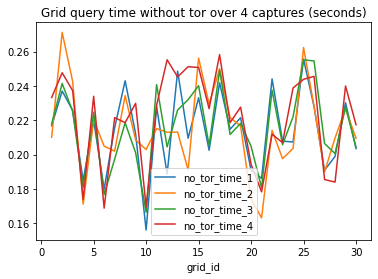
\includegraphics[width=0.25\textwidth]{output.png}
    \caption{Grid query time without tor over 3 captures (seconds)}
    \label{fig:grid_query_no_tor}
\end{figure}
The direction seemed necessary to indicate the link between packet and originator (client/server). The size is noised by TOR's repacketization \cite{noauthor_tor-spectxt_nodate} but we still observed at least 2 kinds of TOR cell sizes (around 500 and around 1k bytes) which can help to see difference between heavy and small payloads. Finally, we found small computation time differences between different grid cell id queries, see Fig. \ref{fig:grid_query_no_tor}, which made us decide to include the timestamp of packets in our trace data. We nonetheless thought that, the computation time delta being in the order of hundreds of milliseconds and communication time in the order of tens of seconds, the TOR network time overhead would noise a lot the application signal.

After calculation, we came to the conclusion that the whole trace would occupy too much space in memory (around 5.2MB for holding one capture of all grid cell id query traces). We therefore chose to group packets by "rounds". As explained, the application answers in "rounds" for the ratings of each PoI. Therefore, instead of storing the size of each packet, we stored the size in bytes of each round (a sequence of packets subsequently going in the same direction). The final shape of our data associates to each label a vector as shown in Table \ref{tab:feature_vec}
\begin{table}[h!]
\begin{center}
\begin{tabular}{l} 
 Number of exchanged packets \\
 \hline
 Duration of the exchange (s) \\
 \hline
 Number of rounds \\
 \hline
 Size round 1 (bytes) \\
\hline
 Timestamp round one (s) \\
 \hline
 ... \\
 \hline
 Size round MAX\_NB\_ROUND (bytes) \\
 \hline
 Timestamp round  MAX\_NB\_ROUND (s) \\
\end{tabular}
\end{center}
\caption{\label{tab:feature_vec}Features Vector}
\end{table}

Where MAX\_NB\_ROUND is the maximum number of rounds observed in all traces. The traces having less rounds are padded with 0 size round and 0.0 timestamp to impact as least as possible the data meaning.
\subsubsection{Classifier training}
For the training part, we used the Random Tree Classifier suggested by the skeleton. We used the library \texttt{RandomForestClassifier} from \texttt{sklearn} and trained using the dataset explained above.

\subsection{Evaluation}

We evaluated using 10-fold cross validation on 4 performance metrics:
\begin{itemize}
    \item Accuracy: the average rate of predictions corresponding to the correct test label
    \item Top 2 accuracy: using the classifier's full prediction distribution for each label, we sorted those in decreasing order of probability. This metric is the classic accuracy but considers as correct a prediction where one of the top 2 predicted labels is the correct label.
    \item Top 10 accuracy: same as top 2 accuracy, this one considers the 10 most probable predicted labels.
    \item True positive: in the same way as the top 2 and top 10, we here took every prediction output by the classifier with a non-null predicted probability. If the correct label is among these predictions, we say it's a true positive (the classifier did not discard the correct option).
\end{itemize}
The results are on average over the 10-folds cross-validation can be found in Table \ref{tab:class_perf}:
\begin{table}[h!]
\centering
\begin{tabular}{ |c|c| } 
\hline
stat & score \\
\hline
\hline
accuracy & 71\% \\ 
top 2 accuracy & 77\% \\ 
top 10 accuracy & 88\% \\
true positive & 97\% \\ 
\hline
\end{tabular}
\caption{\label{tab:class_perf}Classifier performances}
\end{table}

\subsection{Discussion and Countermeasures}

In order to get these results, we tweaked the selected data and classifier parameters. We tried to filter the data columns imported and kept the best results we observed. In the final version, the time and round timestamps columns are discarded as they decreased our accuracy by almost 10\%. We suppose that our data collection not being perfect (the timing of the script changed over the captures, some sleep was introduced etc...), this time data was too noisy. Moreover, as explained, the order of magnitude of computation timing differences observed in Fig. \ref{fig:grid_query_no_tor} orders of magnitude far from the tor network time overhead. Therefore, our supposition is that time correlation in traces mainly come from the transfer time of the transmitted volume and reflects just a noisier data representing the rounds volume.

Finally, we tried but did not keep many modifications on the classifier parameters. We only observed better results when increasing the default number of estimators from 100 to around 260. Further increase did not yield significantly better results. We found that this correlates particularly nicely with the number of features in our training data, which gave us the impression that having at least one tree making decision for every round size feature yields good results.

In order to counter this model, we must come back to our ideas in feature extraction. Indeed, the data has high dimensionality because the sequence of round sizes reveals the number of PoIs and even qualifies them by the size of their ratings. To reduce this, we could, without any utility reduction, shuffle the list of returned PoI by the server so that the client does not query those in the same order every time. Another idea would be to not send the full ratings for each PoI: only some key statistics are necessary and would reduce and normalize the size of every round. Finally, the "round" nature gives information. We could make the client query for multiple PoIs at a time instead of making successive sequential rounds, so that it's harder to observe the signal of a round query.
\bibliographystyle{IEEEtran}
\bibliography{bib}
\end{document}
